\documentclass{article}
\usepackage{graphicx}
\usepackage{subcaption}
\usepackage{url}

\begin{document}

\title{Deploying predictive models with the actor framework}
\author{Brian Gawalt \\
Upwork, Inc. \\
\texttt{bgawalt@upwork.com}
}

\maketitle

\begin{abstract}
 The majority of data science and machine learning tutorials focus on generating
models: assembling a dataset; splitting the data into training, validation, and
testing subsets; building the model; and demonstrating its generalizability. But
when it's time to repeat the analogous steps when using the model in production,
issues of high latency or low throughput can arise. To an end user, the cost of
too much time spent featurizing raw data and evaluating a model over features
can wind up erasing any gains a smarter prediction can offer.

 Exposing concurrency in these model-usage steps, and then capitalizing on that
concurrency, can improve throughput. This paper describes how the actor
framework can be used to bring a predictive model to a real-time setting. Two
case-study examples are described: a live deployment built for the freelancing 
platform Upwork, a simple text classifier with accompanying code for use as an
introductory project.
\end{abstract}

\section{The practice of machine learning}

 Imagine a firm has brought a specialist in machine learning onto a new project.
The firm wants a product which can provide a quality prediction about some
regular event happening in the course of the firm's business. The specialist is
handed a pile of relevant historical data, and asked: Among the new customers
seen for the first time today, who's likeliest to be a big spender? Or: of all
the credit card transactions processed in the last hour, which are likeliest to
be fraudulent? Or: when a customer enters a query into our website's Search
tool, what results should we be returning?

 The specialist starts with the first of two phases of their project. They have
to identify a model that can be expected to fit predictions over both the
historical data and in a way that will generalize to new data. The familiar
version of the steps involved in supervised learning:

\begin{enumerate}
 \item Identify raw source data, and break it down into distinct observations of
the pattern you're trying to learn and predict.
 \item For each raw observation, produce a $p$-dimensional vector of features
and a scalar label.
 \item Split this collection into disjoint training, validation, and testing
sets.
 \item For each candidate model (and/or each hyperparameter value of the
model/models), fit model parameters to the training vectors and labels, and
evaluate the goodness of fit by performing prediction of the validation labels
given the validation vectors
 \item Select the model whose validation-set predictions came closest to the
mark. Use it to then make predictions over the test set. Report this test set
performance to vouch for the predictive model you've generated and selected.
\end{enumerate}

 Note that this first phase doesn't carry an explicit component of \emph{time
urgency}. All else equal, a typical specialist will prefer that the full
sequence complete in six hours, and six minutes is better still. But if it takes
six days instead, nothing \emph{fundamental} to this first phase has been
threatened. The task -- finding a model that generates acceptably accurate
predictions on new data -- is accomplished.

 The second phase is to actually put the model's capabilities to use. Given new
events and observation that need scoring by the model -- is this new customer
likely to be a big spender? is this credit card legitimate? -- the above
featurization and scoring routines need to be run. And in this real-world
deployment, it's likely that there are also some strict constraints on how long
it takes this sequence to run. All predictions go stale, and some use cases need
to act on a prediction within milliseconds of the event itself.

 There are some cases where these latency constraints aren't binding. The exact
same featurization and scoring routines used to generate and validate the model
can be re-run fast enough on new data to produce useful predictions. But this
paper focuses on the cases where timeliness requirements exclude the use of the
same software developed in the first phase as the backbone of the second phase.
What can a lone machine learning specialist do to retool their sequence to run
in a production environment?

\subsection{Moving to production}

 If the original software, used to generate and validate the predictive model,
is suffering from too-low throughput in producing new predictions, one path
forward could be to incorporate more concurrent processing. The three steps to
prediction (gathering raw materials, featurizing those materials into vectors,
scoring the vectors) can transition from a serial sequence to a pipeline.

  Figure~\ref{fig_pipeline} demonstrates a modification of the scoring task flow, producing
predictions of $N$ events in a sequential and a concurrent pattern.  This
pipeline offers a few advantages. Scores are produced with less delay after the
raw material gathering (useful in case the information in that material is at
risk of going stale or out of date).

\begin{figure}[h]
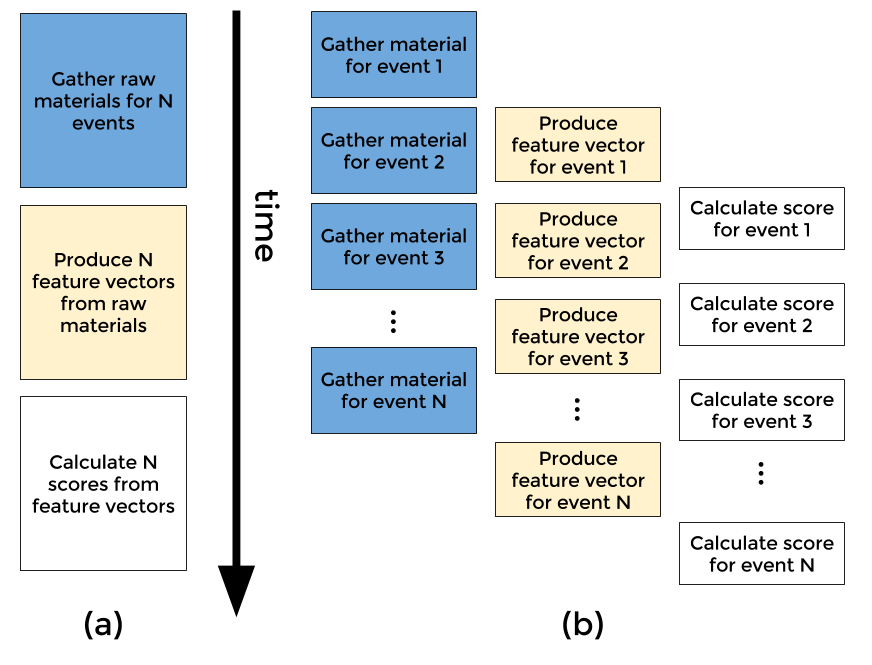
\includegraphics[width=0.6\textwidth]{fig/tex/pipeline.png}
\centering
\caption{(a) The scoring procedure performed serially. (b) The individual tasks
for each event to be scored performed in a concurrent pipeline.}
\label{fig_pipeline}
\end{figure}


 Most importantly, this redesign provides a clear path forward to speed-up in
completing all $N$ scoring tasks. If a system can genuinely perform the
concurrent tasks in parallel, as a multicore system might, one can easily
picture adding ``clones'' of this pipeline simultaneously processing more and
more partitions of the $N$ events.

\subsection{Complexity costs}

 It can be difficult to put together, from scratch, a high-performance
concurrent computing system. It's easy to fall into traps of false sharing,
deadlocking, and other difficulties. It's not impossible, but it's definitely
tricky and time-consuming, and building a new concurrent system for a single
project might fail a cost-to-benefits ratio test.

 Fortunately, lots of great work has produced platforms to take this plan to a
truly wide scale implementation. Apache Storm~\cite{apache_storm}, 
Apache Spark (especially its Spark Streaming library)~\cite{apache_spark}, 
and Twitter's Heron~\cite{kulkarni2015heron} all try to distribute this kind of 
event-driven computing across multiple machines to ensure the highest 
possible throughput.

 Unfortunately, they're complicated systems. Familiarizing oneself with the API,
and managing the underlying infrastructure, requires considerably more expertise
above and beyond that of our original model in Figure 1(a). If spreading the
load over multiple machines is the only way to meet the required service level
of the prediction system, this additional complexity will have to be met with
additional resources: maybe the firm will have to start allocating more
engineers in addition to more hardware, to what originally was a project of just
the single machine learning specialist.

 This paper is here to specifically recommend a midpoint between a from-scratch
concurrent framework and the mega-scale offerings. The actor framework offers a
simple way to reason through concurrent problems, while still being flexible
enough to accommodate a variety of approaches to any one problem. The ease

 From here, this paper presents a case study where an actor framework was key to
bringing a predictive model to production. It interleaves this story with a
summary of what an actor framework entails, as well as a description of the
framework implementation in the Scala library Akka. It concludes with a reiteration
of the advantages (and disadvantages) the actor framework offers and a
discussion of why comfort with actors can help machine learning specialists with
their work and careers.

\section{Case Study: Predicting worker availability at Upwork}

 Upwork is an online labor platform, connecting freelancers and clients for
internet-enabled remote work. There are several patterns for how these work
arrangements are struck\footnote{Freelancers can send proposals for a client's
publicly posted job opening; groups of freelancers form agencies to share many
client workloads; clients and freelancers, already working together outside the
platform, moving their relationship onto Upwork to take advantage of the site's
payment processing, escrow, or other services}, but one important avenue
involves a client using the platform's search engine to discover new freelancers
they think would be well suited to the project the client has in mind.

 When the client issues a query, e.g., ``java developer'', ``restaurant menu
design'', ``paralegal'', they expect to see a result set filled with freelancers
with relevant experience who are likely to perform well on a new assignment. The
client can then invite any of these freelancers to interview for an open
position.\footnote{Upwork sees the two actions happen in both orders. Sometimes,
clients post a job opening, then go searching for freelancers to invite to
interview; other times, the client starts by searching and browsing freelancer
profiles, and creates the job post once they see someone they'd like to work
with.}

 This adds a third requirement to the query's result set: listed freelancers
should not only be relevant and high-performing, they should also be receptive
to an interview invitation at the time of the query. If the system returns a
list of the same ten excellent freelancers are returned for every search for
``wordpress template,'' it's a recipe for those ten freelancers being deluged
with opportunities they're to busy to fill (and for the freelancers ranked just
outside that top ten being unreasonably starved for job invitations).

 There was an existing heuristic in place to try and capture this, but it was
felt a learned model trained on historical data could easily provide higher
accuracy.

\subsection{Building the predictive model}

 If the system should only show freelancers available to interview, how should
we estimate freelancer availability? This question can be gently reformulated
into a question of binary classification: ``If Freelancer X were to receive an
invitation to interview right now, does their recent use of the site suggest
they would accept that invitation, or would they instead reject or ignore it?''

 A logistic regression model can help answer this question. Each invitation sent
from a client to a freelancer was treated as an example event, labeled as a
positive class member if it was accepted and negative otherwise. (There were
roughly one million such examples within a relevant and recent time frame.) The
goal would be to link the freelancer's recent site activity -- within the month
prior to receiving the invitation -- to the outcome of an acceptance or
rejection of the invite.

The raw materials, and derived features, came in four main varieties:

\begin{description}
 \item[Job application/invitation history] In the previous day, how many job
applications did Freelancer X create? How many invitations did X receive? How
many of each were cancelled by the client, or by the freelancer? How many of
each led to filled jobs? Answer these questions again for the time periods: two
days, four days, seven days, 14 days, and 30 days.
 \item[Hours worked] How many hours has Freelancer X billed to any client in the
preceding day? two days? ... thirty days?
 \item[Server log history] In the previous one/two/.../thirty days, how many
times has Freelancer X visited pages under the ``Job Search,'' ``Message
Center,'' and ``View Contractor Profile'' sections of Upwork.com?
 \item[User profile] How many jobs has the freelancer worked in each of Upwork's
job categories (e.g., Web Development, Graphic Design, Data Entry)? What is
their stated preference for receiving more invitations at this time (``I am
available,'' vs. ``I'm not currently available'')?
\end{description}

 These raw materials (along with a few other sources) could be harvested from
three services: a Greenplum relational database for assembling job application
and hours-worked data, and an Amazon S3 bucket for the server logs. The
user-profile information was an interesting case: the historical state of the
profile was logged to a table in Greenplum with each invitation, but a
freelancer's present profile state required a call to an internal service's REST
API.

 Assembling these feature vectors and performing a training-validation-testing
split led to a model with a test-set AUC metric of around 0.81. This
sufficiently outperformed the existing heuristic's accuracy, and the model was
deemed ready for production use. Freelancers would start receiving scores from
the model, putting them into buckets of low, medium, and high availability
(i.e., high propensity to accept an invitation to interview at this time).

\subsection{Throughput constraints in production}

 An interesting aspect of this modeling task is that hour to hour, any
individual freelancer's availability score might swing considerably. Someone who
looked dormant three hours ago could decide to log back onto Upwork and start
engaging in eager-for-work behavior, sending out job applications and polishing
their profile. Another freelancer's behavior might cause a sudden transition
from looks-available to looks-overbooked. The more frequently each freelancer
could be scored, the more faith Upwork could have that the bucketing used by the
search engine was using reliable information. Keeping freshness of the raw
material data under four hours was considered a reasonable goal.

 Generating those scores meant providing the routine with those four families of
raw material. When developing the model using historical data, all four could be
gathered and processed in bulk, in advance of the featurization and scoring
routines. In a production setting, this remained the case for data from S3 and
Greenplum: all that relevant information, for all registered freelancers, could
be collected in under an hour.

 However, user profiles posed a challenge: given other demands placed on it by
other Upwork.com systems, the internal user profile service could only afford to
return one user profile every 20 milliseconds to the availability scorer. Any
more rapid than that threatened the health of the service. That placed a maximum
of 4.3 million scores to be produced per day, one for each up-to-date profile
request. With six million total registered freelancers, this put the squeeze on
the preliminary goal of every-freelancer, every-four-hours.

\subsection{Concurrency under the actor model}

 A direct re-use of the routines in the model generation software would involve:

\begin{enumerate}
\item bulk collection of the job application and worked-hours data,
\item bulk collection of the server log data,
 \item bulk collection of as many user profiles as possible before the data from
(1) and (2) could be considered stale,
 \item featurization and scoring of each freelancer whose profile was collected
in step (3).
\end{enumerate}

 Steps (1) and (2) combine to a total of about 40 hours of collection and
processing time when performed sequentially. Keeping a buffer of 5 minutes aside
for Step (4)'s vectorization and scoring (and saving those scores to disc), that
means a 4 hour cycle will involve 195 minutes of harvesting user profiles in
Step (3). That means an amortized rate of 146,250 scores produced per hour. 

The fastest rate possible (one every 20 ms, as limited by the necessary
contributions from the user profile service) would mean 180,000 scores per
hour. That leaves room for a potential 23\% improvement in throughput
by moving to a system where user profiles are harvested concurrently
alongside the other routines. This potential upside increases as the
stringency of the data-freshness guarantee is increased from four
hours, to two hours, to one.

\subsubsection{The actor model}

The actor model makes it easy to architect a concurrent version of the
availability system. An actor framework involves three components:

\begin{description}
\item[The Actors] A collection of objects, each holding a message queue, some 
private state, and some private methods. This state is can only be updated, and
these methods can only be called, by the actor object itself, and in response to 
receiving a message from some other actor. The response an actor takes to each
message is fully completed before it begins its response to the next message.
\item[The Messages] Simple, immutable objects that contain information or 
instructions one actor wants another actor to notice. 
\item[The Execution Context] The harness which ensures that each dispatched 
message reaches the right actor queue, the computation each actor calls for is
completed in order, and that the overall workload is balanced as evenly as possible
over the available hardware resources. This system also provides methods for
creating new actors, as well as for setting up a timed schedule to dispatch
messages at regular intervals to any actor.
\end{description}

This message-passing version of concurrency avoids the race conditions and
other difficulties that can arise from many execution tasks sharing mutable state.
Anything mutable is isolated inside individual actors, who only share with each
other immutable message objects.

The actor model rose to prominence in an artificial intelligence context thanks to
work from Hewitt, Bishop, and Stieger.~\cite{hewitt1973ijcai} It's true that compared
to classical imperative programming ``it imposes a major mind shift in software
design,''~\cite{korland2011thesis} it's a comparatively small leap with respect, with
fewer pitfalls for novice (or harried) developers to hazard.

\subsubsection{The concurrent availability system}

% TKTK Why not just make a bunch of queries to Greenplum???
% A: Cuz that's EVEN WORSE, like minutes per score

The family of actors defined for a concurrent availability prediction system uses a
hub-and-spoke arrangement, with a single lynchpin actor in charge of featurization
from a freelancer's raw data. Three ``historian'' actors are in charge of polling the 
higher-bandwidth Greenplum and S3 sources, and another is in charge of (rapidly)
polling the user profile service; all four send their findings back to the central
featurizer for storage as state variables. A sixth actor receives (freelancer ID, feature
vector) pairs from the featurizer, applies the model, and stages these scores to be
bulk uploaded back to Greenplum, where the rest of Upwork's freelancer search
systems can make use of it.

% TK TK Maybe move this to an appendix?
In more detail:

\begin{description}
\item[The featurizer] The central hub of the actor system: the featurizer keeps track of
each freelancer's worked-hours, job application, and server log information,
updating this background data whenever an update is received from a Historian.
Whenever a freelancer's information is received from the User Profile Fetcher -- that 
profile holding the final piece of information needed for a complete feature set --
the featurizer sends the freelancer's feature vector to the scorer-exporter.

\item[The historians] Each is responsible for polling a different kind of raw
material resource. The execution context is given a timing schedule for
each, and periodically sends them ``poll for new data now.''
	\begin{description}
	\item[Worked-hours historian] Fetches worked-hours records from 
	Greenplum at a schedule of once per hour, forwarding the results found
	to the featurizer.
	\item[Job applications historian] Fetches the job application record from
	Greenplum at a schedule of once per hour, forwarding.
	\item[S3 historian] Fetches the latest server logs at a schedule of once per hour,
	forwarding them to the featurizer.
	\item[User profile fetcher] Every 20 milliseconds, requests and processes user 
	profile data from Upwork's internal service, passing the results back to the featurizer.
	\end{description}

\item[The scorer-exporter] Waits to receive from the featurizer  a freelancer ID, and a
vector of features capturing that freelancer's recent use of the Upwork platform.
It then applies the (previously trained) logistic regression model to the features,
generating a ``odds-of-accepting-an-interview-invitation'' score for that freelancer.
The scorer-exporter stores as many of these as it receives in one hour, then
uploads the large collection all at once to a table in Greenplum where it can be
read by the rest of the Upwork backend systems and incorporated into search
rankings.

\end{description}

This family of actors, along with arrows indicating the principal flow of information 
from raw material, to feature vector, to availability score, is depicted in
Figure~\ref{fig_av_system}. It's a 

\begin{figure}[h]
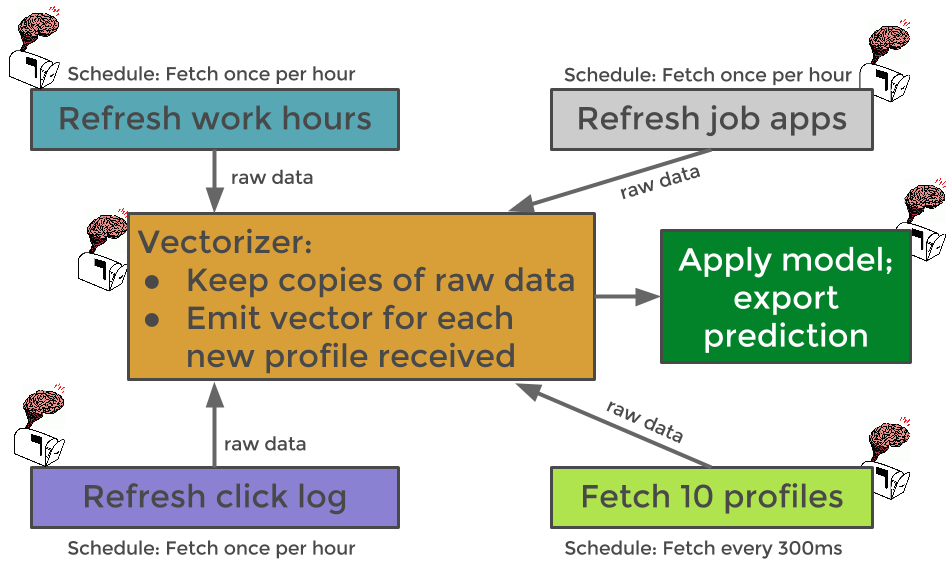
\includegraphics[width=0.7\textwidth]{fig/tex/availability_system.png}
\centering
\caption{The actor system for freelancer availability scoring. Each actor can be thought of
as a mailbox, queuing up messages, with a little brain, holding memories and reacting to 
those messages one by one.}
\label{fig_av_system}
\end{figure}

By dividing responsibility for the full scoring pipeline across several distinct workers,
the execution context is able to take their concurrent operations and schedule them
for the operating system to perform. When the underlying machine offers multiple
CPUs, this can mean the actors operate simultaneously, allowing for the 
latency-reducing speed ups we were hoping for. And the single-file
processing of messages we avoid problems where, e.g., one step in the scoring 
procedure tries to read its stored worked-hours data at the same time another
step is updating that same data -- trying to square this circle from scratch
can easily result in code that deadlocks, livelocks, or just plain drops data.

Figure~\ref{fig_avail_serial} depicts the order of operations from our original,
sequential scoring system, where raw material gathering, vectorization, and
scoring happen one after another, repeating once an hour. Time spent gathering
the Greenplum and S3 resources takes away from the rate-limited use of
the user profile service.

Figure~\ref{fig_avail_concur} demonstrates the concurrent availability scorer
run on a four core machine. The execution context is able to provide parallel
execution of actor routines, meaning the user profile historian never \footnote{
This may be a little generous: the Java runtime environment itself may preempt
the execution of one or more actor's operations in order to execute services like
garbage collection.} needs to take a break to let the other raw material harvesters 
use the execution thread. The rate of availability score production can be maxed out 
by taking full, round-the-clock advantage of the rate-limited resource.

\begin{figure}
\begin{subfigure}{.5\textwidth}
	\centering
	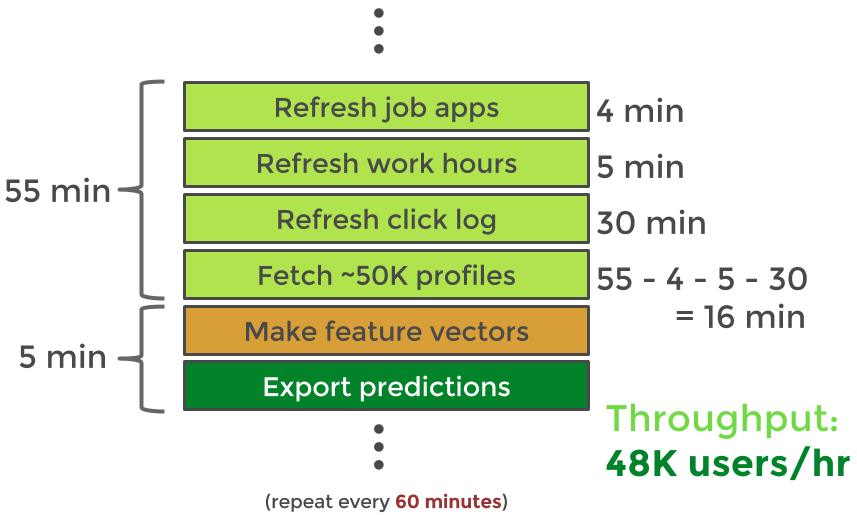
\includegraphics[width=.95\linewidth]{fig/tex/availability_serial.png}
	\caption{Sequential operation}
	\label{fig_avail_serial}
\end{subfigure}
\begin{subfigure}{.5\textwidth}
	\centering
	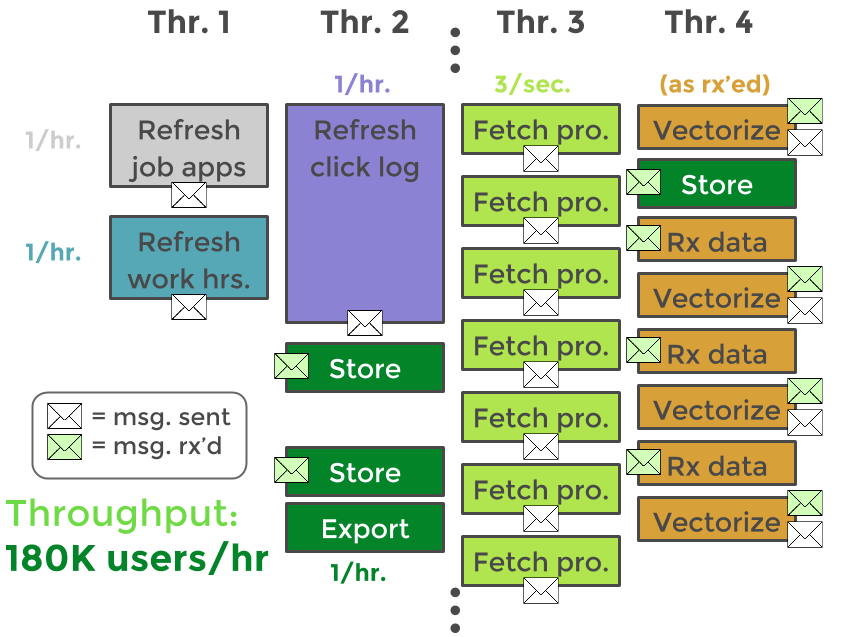
\includegraphics[width=.95\linewidth]{fig/tex/availability_concurrent.png}
	\caption{Parallel operation}
	\label{fig_avail_concur}
	\end{subfigure}
\caption{The computation cycle for availability in its sequential and concurrent
formulations, on a four-CPU system. When data is kept to within one hour of
freshness, the actor model provides an approximately 3.75-fold increase in
throughput}
\label{fig_avail_serial_concur}
\end{figure}

The actually-implemented availability system, now running as a service on 
Upwork's backend, achieves this same rate of freelancer score production.

\section{Case study: a text classification API}

As a hands-on demonstration of powering a machine learning service with
the actor framework, a repository of code has been put online as a companion 
to this paper at \url{https://github.com/bgawalt/papis-akka-demo}.~\cite{gawalt_papis_demo}
The project is an online learner, a text classifier trained one example at a time
to distinguish between positive and negative class documents (e.g., spam 
versus valid messages).

It is implemented in Scala, making use of the Akka~library~\cite{akka_doc}
to handle the execution context and actor classes, and the Spray~library~\cite{spray_doc}
to connect that execution context with HTTP requests from the outside world.

\subsection{Scala, Akka and Spray}

Scala is high level language, designed to allow for easy productivity when
developing in both functional programming and object-oriented styles. The
Scala language allows developers to define \texttt{trait}s, ways to partially 
define class features. Declared attributes can be implemented right
along with the \texttt{trait} definition itself, or they can defer the implementation
until the trait is finally used to build a legitimate \texttt{class}.

They're much like Java's \texttt{interface}s, with the added benefit of mixin 
capabilities -- several \texttt{trait}s can be defined independently with their own
 methods and fields, then combined arbitrarily to create new subclasses sharing
 the union of their attributes.

The Akka library provides a \texttt{trait} called \texttt{Actor}. To define an actor, 
declare a new \texttt{class} which extends \texttt{Actor}, which will require you to
implement the method \texttt{receive}. This method is of type \texttt{PartialFunction[Any,~Unit]},
exactly as we'd expect: the actor can receive any kind of message, and then does 
something. The \texttt{match} keyword makes it easy to encode reactions to different
expected message types, and provide a default ``unexpected command'' behavior.

\subsection{Text classification servers}

The demo project involves two approaches to the same binary classification task,
implemented as two separate API servers: \texttt{LoneLearnerServer} and
\texttt{PackLearnerServer}. These APIs are backed by two types of actor: the request
parser and the learner. 

The request parser, one per server, inherits from Spray's \texttt{HttpServiceActor},
whereby HTTP requests to a particular socket can be forwarded to the parser's
\texttt{receive} method as a \texttt{RequestContext} object. This request context
contains useful information, like the URL of the resource requested, and has a
\texttt{complete} method which should be invoked to send a response to the
client via Spray's HTTP mechanisms.

The parser can decode the requested URL and then forward instructions, along with
the context to be completed, to the second actor in the system: the learner. Via this 
API, the learner can perform six tasks: score a new document based on the current 
model state; update the model state when given a document and a positive or negative 
class label; report its current state as a string; reset itself to it's original, 
zero-observations state; synchronize with fellow learners by transmitting information
about recently-seen observations, or incorporating that information received from another
learner.

The \texttt{LoneLearnerServer} has only two actors: one parser, listening to HTTP on
a particular socket, and a learner, waiting to receive new documents to judge or labelled
documents to learn from. Figure~\ref{fig_txt_cls_sng} lays out the basic execution flow.
There's a risk that too many requests received in rapid succession could cause steadily
longer delays between client request and response.\footnote{In practice, it seems
fairly rapid even with this obvious bottleneck -- on a two-core machine, the system was
able to process 20,000 predict-then-update cycles in around 60 seconds, or about 
1.5 milliseconds per instruction to the learner.}

\begin{figure}[h]
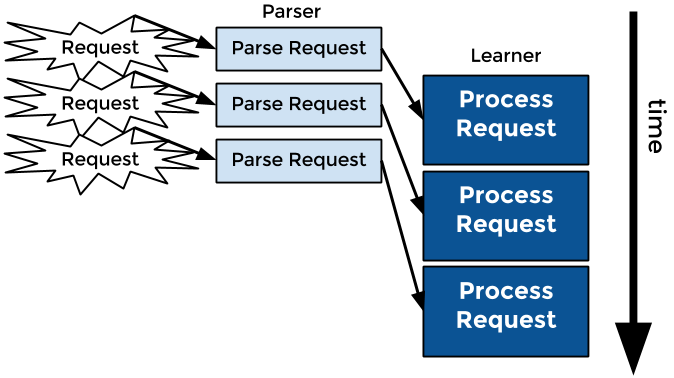
\includegraphics[width=0.7\textwidth]{fig/tex/single_txt_cls.png}
\centering
\caption{A text classifier system with a lone learner. The learner, with its more
computationally intensive tasks, is a potential bottleneck, and latencies can increase as
requests pile up.}
\label{fig_txt_cls_sng}
\end{figure}

To break this bottleneck, \texttt{PackLearnerServer} has a single parser working
with $N$ learner actors. Each HTTP request parsed can be routed to a single learner,
selected in a one-after-the-other sequence, or selected pseudorandomly (such as by 
taking the request's hash value modulo $N$), spreading the computational load and
increasing the odds that the selected learner fielding the request will be unoccupied and
ready to work at the time of the request. 

The drawback is that when a new labelled document is observed, it can only update
the model housed in the selected learner's state. Predictions made by the other
learners in the pack won't be able to benefit from the knowledge gained from the 
update. To patch this, learners are able to send each other update messages
after a certain number of observations. This synchronization pulls them offline, unable
to respond to new requests until the updates are incorporated. 

The machine learning specialist can judge how to trade more frequent updates (and 
potentially longer delays between request and response) for greater fidelity to the full 
collection of observed documents. Figure~\ref{fig_txt_cls_dbl} depicts an example of 
this system's execution of requests.

\begin{figure}[h]
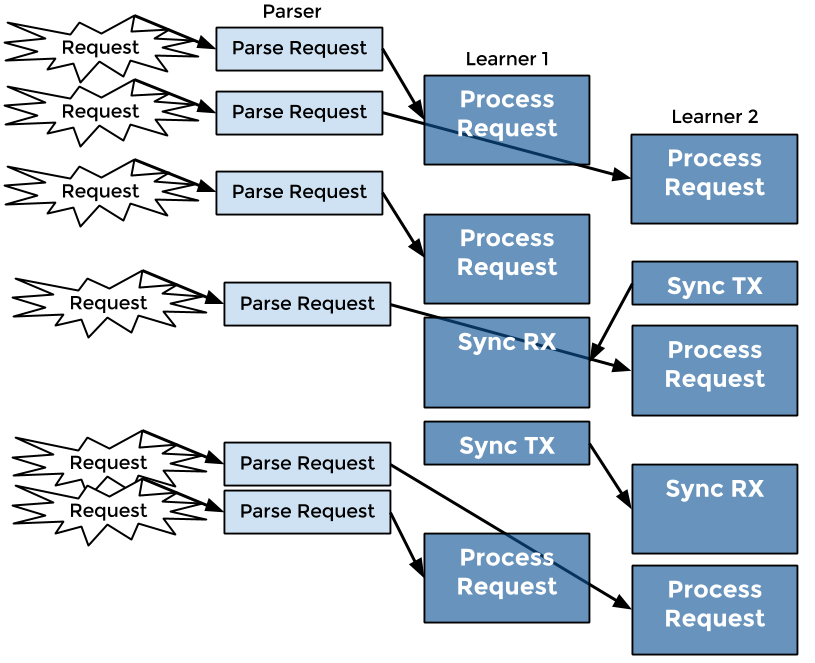
\includegraphics[width=0.7\textwidth]{fig/tex/double_txt_cls.png}
\centering
\caption{A text classifier system with multiple learners. Request latency can be reduced
by sharing the load, though a trade-off has to be made: learners can stay in the dark 
about recent observations for longer periods (possibly issuing noisier predictions), or 
more time can be spent synchronizing models between learners (possibly delaying 
new requests). Note the order in which requests are completed may not match the 
order in which they were issued.}
\label{fig_txt_cls_dbl}
\end{figure}

\section{Conclusion}

Data science and machine learning are growing as fields and professions, 
expanding into new domains. That necessarily means engaging firms who 
find the whole field unfamiliar; and unfamiliarity can inspire risk aversion. 
These firms in particular are going to greatly appreciate it when a specialist
demonstrates a production-ready model at minimal cost, including infrastructure
costs, engineering person-hour costs, and maintenance costs.

Exposing concurrency yields efficiencies and reduces costs for any service.
Machine learning and data science products benefit especially from the actor 
framework. It is straightforward to take the standard procedure -- gather raw data, 
produce features from that data, and score those features -- and define a collection 
of actors. That simplicity generates savings in engineering and maintenance efforts.

Upwork was able to take an underperforming sequential software routine, port the
particular components to one actor each, and build a system which achieves the
maximum possible scoring throughput with much-improved ``freshness'' guarantees.

The true benefit of the actor framework is its simplicity. The \texttt{LoneLearnerServer}
text classification API, built on the well-designed Spray and Akka libraries, is under 
250 lines of code. And other languages offer their own actor libraries.

For Java, there's the Quasar platform~\cite{quasar_doc}, as well as a Java API for
Akka. For C++, there's CAF, The C++ Actor Framework~\cite{charousset2014caf}.
For Python, Pykka~\cite{pykka_doc} (though to take advantage of parallelism,
your program may benefit from Jython~\cite{jython} and it's lack of global interpreter
lock). For Ruby, consider Celluloid~\cite{celluloid_doc} (as with Python, consider 
JRuby~\cite{jruby_doc} or Rubinius~\cite{rubinius_doc} to enable thread-level
parallelism).


Having the simple version of a predictive API up and running
makes it easy to expose and capitalize on greater amounts of concurrency:
\begin{itemize}
\item Which actor routines can swap their I/O library for a non-blocking equivalent
(freeing thread resources for another actor to use)? 
\item Can the workload be smoothed by managing duplicate actors (as with
 \texttt{PackLearnerServer} in our example), or by spawning new actors 
 on-demand? 
\item More ambitiously, can we start building distributed networks of actors, passing 
info and sharing tasks?
\end{itemize}

There is a scale where the actor framework and its concurrency is overkill.
Some machine-learned models only needs to produce new scores 
infrequently enough -- a new batch overnight, say -- that allows for the exact
same routines to be used ``in the wild'' as were used for designing, validating,
and testing the model ``in the lab.'' The machine learning specialist might be
of more use moving on to generate a new or better model, than to rig up

There is a scale where an actor framework starts requiring greater and greater
care and maintenance. Without backpressure, overstuffed mailboxes can cause 
fatal out-of-memory errors. Timed-out operations need to recover gracefully.
As these problems mount, the value proposition of large-scale platforms like
Spark and Storm become more compelling.

The actor framework helps the machine learning specialist bridge the gap 
between these scenarios. It is capable enough to support medium-scale
applications, especially given the present affordability of four, eight, sixteen
core systems. It is simple enough that the specialist can assemble the
concurrent solution on their own: a production deployment from the same
person who designed the model.

Empowered, self-sufficient data scientists are going to continue to push the 
frontiers of their profession. They should consider adding the actor 
framework to their toolkit.

\bibliography{papis_akka_demo_bib}
\bibliographystyle{plain}

\end{document}









